\chapter{Introduction to the technologies used} \label{technologies introduction}

This chapter includes introduction on the technologies chosen for the POC (proof-of-concept) project.
The technologies and their roles in the project are explained in the amount of detail necessary.

The project is built as a POC implementation of a GDPR-compliant patient data storage for a healthcare organization.
The technologies are chosen after evaluating their fit for the project and their familiarity for the organization after discussing the choice with them. 
The chosen technologies are as follows:
\begin{itemize}
    \item Google Cloud Platform
    \item Terraform
    \item PostgreSQL
    \item Node.js
    \item TypeScript
    \item Docker
\end{itemize}

\section{Google Cloud Platform}

There are many providers in the cloud computing space.
For example, Amazon, Google, Microsoft, Rackspace and DigitalOcean have grown to provide services for numerous users.
Different providers offer similar products, but the implementation details and how they work vary significantly.
\cite{mastering-google-cloud} 

Google Cloud Platform (GCP) is a selection of cloud computing services provided by Google.
GCP started as Google App Engine framework for hosting web applications from Google's data centers and grew from there to offer a wide variety of services.
Nowadays, it is one of the largest cloud computing platforms, but still behind Amazon Web Services (AWS) and Microsoft Azure in market share.
Google promises the users of its cloud platform 99.95 \% reliability, which they achieve by building safety systems around in their applications by assuming any of the parts can fail.
Google is also running constant performance and load tests on their services, finding and troubleshooting problems proactively.
\cite{mastering-google-cloud}
Different categories of services offered GCP are visualized in Fig \ref{fig:google-cloud}.

\begin{figure}[!htb]
\centering
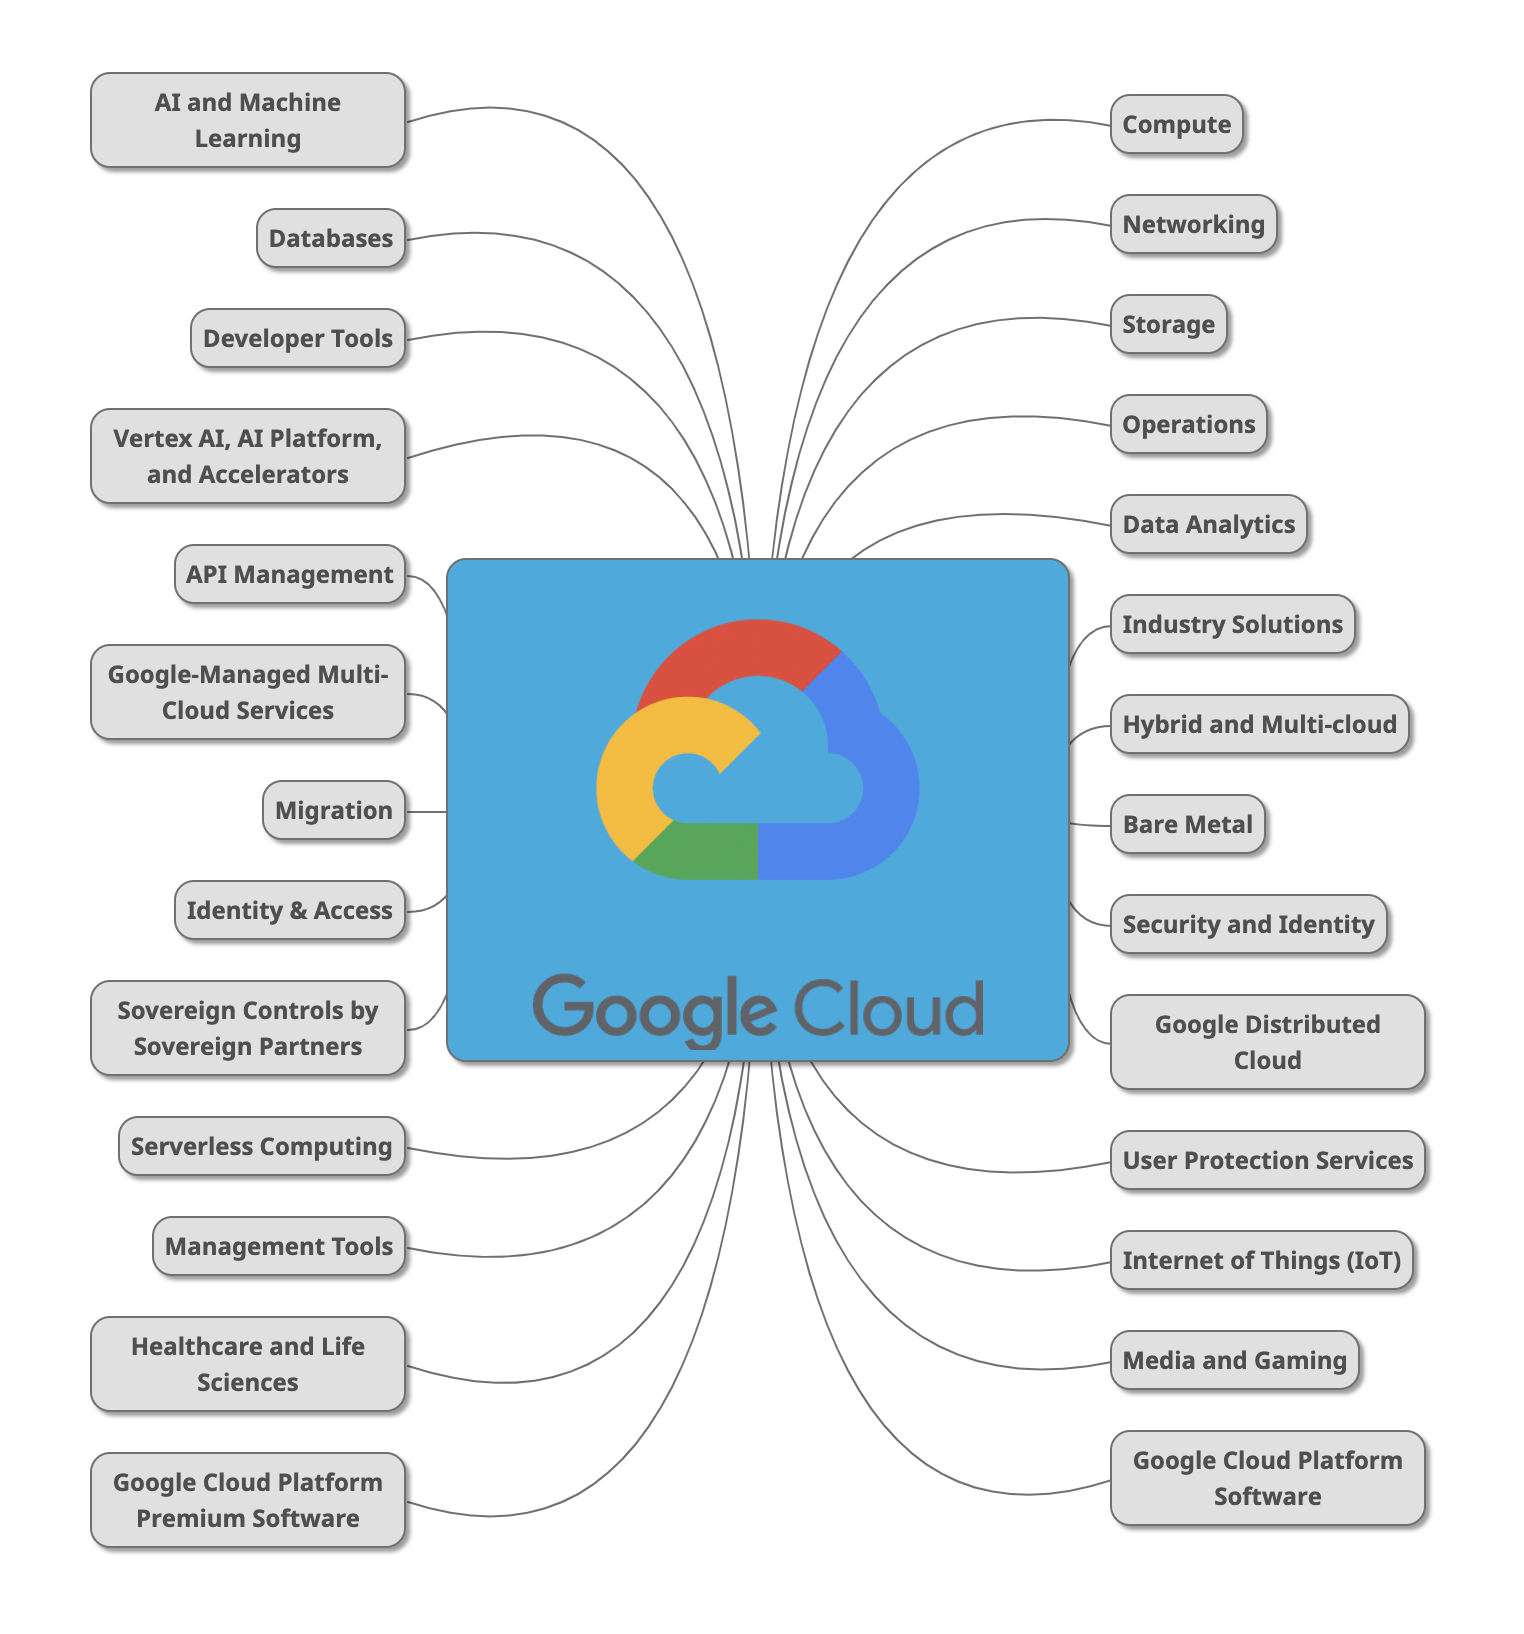
\includegraphics[scale=0.55]{googlecloud}
\caption{Visualization of the categories of services Google Cloud Platform offers}
\label{fig:google-cloud}
\end{figure}

The most straightforward way to manage the services provided by Google Cloud Platform is the web-based console served at console.cloud.google.com.
Google also offers tooling called the Cloud SDK for interfacing with Google Cloud Platform.
The SDK supports interacting with Google Cloud Platform products and services using client libraries for Java, Python, Node.js, Ruby, Go, .NET and PHP.
The SDK also includes a command line tool called the Google Cloud CLI for managing GCP services.
\cite{googlecloud}

Google Cloud Platform offers many options for building cloud based services.
GCP offers compute, storage and networking services along with many others.
For example, Google App Engine is a service for hosting a fully managed server-side application.
Cloud SQL is Google cloud's offering for a fully managed PostgreSQL database.
Cloud DNS is their platform for managing all things DNS as well as registering and managing domains.
These are only a few examples of the services provided by Google Cloud Platform.
The specific services chosen for the POC are explained in more technical depth in the next chapter.
\cite{googlecloud}

\section{Terraform}

In place of managing cloud computing resources using a web-based console, a client library or a command line interface, there is another option.
Infrastructure as Code (IaC) is defined as building infrastructure in a declarative way.
Instead of clicking through a graphical interface or building a script to tell a computer how to build the infrastructure, IaC languages are used to define what the infrastructure is, and let the IaC technology handle building and changing it.
IaC technologies have the benefit of making the infrastructure more replicable and easier to version and document.
\cite{terraform}

Terraform is an open source infrastructure as code tool created by Hashi\-Corp.
Terraform as a technology consists of multiple tools: Terraform CLI, Terraform Cloud and Terraform Enterprise.
In the scope of this thesis, the most relevant tool is Terraform CLI: a command line tool launched using the \verb|terraform| command.
Terraform CLI can be used for any action the developer would do such as \verb|terraform plan| and \verb|terraform apply|.
Terraform uses HashiCorp's own Hashi\-Corp Configuration Language (HCL) as its main interface.
HCL aims to be both: a human- and a machine-readable configuration language for use with command line tools.
\cite{terraform}

Terraform allows building both cloud and on-premise infrastructure.
Terraform does not specialize in any technology, but instead it allows for the use of so-called providers for many different platforms and technologies.
At the time of writing HashiCorp and the Terraform community have released over 1700 different providers on the Terraform registry\footnote{https://registry.terraform.io/} including for example Amazon Web Services (AWS), Azure, Google Cloud Platform (GCP), Kubernetes, Helm and many more.
Terraform providers interface with different cloud platforms and other services via their application programming interfaces (APIs).
A provider can be created for virtually anything that has an accessible API.
\cite{terraform}

The Terraform workflow consists of three main steps.
First, the developer writes the configuration which defines the infrastructure.
The second step is the plan stage where the developer reviews the changes Terraform will make to the infrastructure, including things that will be created, updated or destroyed.
Third, the developer applies the planned changes to the actual infrastructure.
Terraform will handle changing the infrastructure in the correct order and updating its own internal state file.
Destroying the infrastructure can be considered the fourth step after the infrastructure has served its purpose.
\cite{terraform}
The Terraform workflow is visualized in Fig \ref{fig:terraform-workflow}.

\begin{figure}[!htb]
\centering
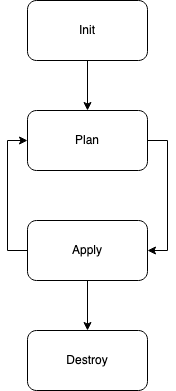
\includegraphics[scale=0.8]{terraform-workflow}
\caption{Visualization of the steps included in the Terraform workflow}
\label{fig:terraform-workflow}
\end{figure}

Terraform has an abstraction called a \textit{module}.
A module is a lightweight container that includes multiple resources that are used together.
Using a module makes declaring the architecture itself easier, without declaring the physical parts themselves.
A module can also take input variables to allow for building configurable and reusable building blocks.
It can return output values as well, which can be used as arguments elsewhere.
\cite{terraform}

\section{PostgreSQL}

PostgreSQL is an open-source object-relational database management system.
It is designed to handle a large variety of workloads ranging from single servers to data warehouses and huge web services.
It has a history spanning over 30 years which gives it a reputation as a powerful, reliable, robust and performant database.
PostgreSQL supports a large part of the SQL standard and offers many more modern features, such as complex queries, foreign keys and updatable views.\footnote{Foreign keys are used to validate the existence of an entry and store a reference to it in another database table. An updatable view is a database view that can be updated similarly to a regular table.}
\cite{postgresql}

PostgreSQL is based on a database system developed at the University of California at Berkeley Computer Science Department: POSTGRES, Version 4.2.
POSTGRES pioneered many new concepts for database systems.
PostgreSQL is an open-source successor of POSTGRES.
It is released under a very liberal license allowing for use in any sort of application, be that private, commercial or academic.
\cite{postgresql}

The PostgreSQL database runs on macOS, Windows, Linux, FreeBSD and Open\-BSD. \cite{postgresql}
In addition to running PostgreSQL on the user's own server hardware, many cloud providers sell managed services for hosting PostgreSQL.
For example, The Google Cloud Platform includes a fully-managed service for hosting and administering a PostgreSQL database called the Cloud SQL.
\cite{googlecloud}

\section{Node.js}

Node.js is a runtime environment for JavaScript which is designed to build scalable network applications.
Node.js is a cross-platform environment which can be used to run JavaScript outside the browser for use cases such as command line tools and server-side applications.
It is an open-source project built by the OpenJS Foundation and runs on Google Chrome's V8 JavaScript engine.
Node.js was first released in 2009 and has gained huge popularity among all types of users ever since.
\cite{nodejs}

Node.js uses an event-driven architecture for building applications.
It executes code concurrently, such as allowing for multiple connections.
This is in contrast to the more common thread-based model.
The concurrency model makes building scalable systems with Node.js very reasonable, as user will not have to worry about deadlocking.
However, this does not mean Node.js can not take advantage of multiple cores in your environment.
\cite{nodejs}

Node.js is designed to be modular.
It can be extended using packages installed via Node package manager (npm).
Npm is a command line tool designed to make installing packages quick and easy.
Npm's registry has grown to become the world's largest software registry.
The registry can be browsed using its website at https://npmjs.com.
\cite{npm-docs}

Express is a web framework for Node.js.
It is designed to be fast, unopinionated and minimalist.
Express makes building solutions such as APIs for web and mobile applications simple and flexible.
Express by itself only includes a thin layer of web fundamentals required, but it can be expanded with any of Node.js libraries.
Requests to the Express application can also be intercepted and handled with a method called \textit{Middleware}.
\cite{expressjs}

Pg-promise is another example of a Node.js library built to interface with PostgreSQL.
It is built on top of node-postgres.
The name pg-promise comes from it only first adding promises as its sole feature, JavaScript's solution for handling asynchronous computation.
Nowadays the library adds a lot of other features as well.
The features it adds include for example automatic connections, automatic transactions and improved query formatting.
\cite{pg-promise}

\section{TypeScript}

TypeScript is a programming language created by Microsoft.
TypeScript extends JavaScript's syntax by adding types to it.
It is a strict superset of JavaScript, which means all existing JavaScript code is also valid TypeScript code.
JavaScript already provides primitive types such as string and number, but does not do any type checks with these.
TypeScript allows describing types explicitly and inferring types from constants.
The compiler then checks for type errors before ever running the code.
TypeScript promises to give the developer better tooling such as tighter integration with the editor.
It also promises to allow for finding bugs earlier on in the development.
\cite{typescript}

TypeScript compiles to JavaScript and can run anywhere JavaScript runs. The possible execution environments include for example web browsers and Node.js.
JavaScript already uses types such as \texttt{string} and \texttt{number}, but it does no checking on how variables are assigned.
TypeScript does this and allows defining more complex types.
\cite{typescript}

TypeScript uses all the same types JavaScript already has, but also adds a few more.
For example, the \texttt{any} type allows anything to pass into the variable.
TypeScript also has support for defining more complex types.
An \texttt{interface} can be used to define the shape of an \texttt{object}.
The \texttt{type} syntax can be used to create even more specialized types, such as unions and \texttt{string} or \texttt{number} literals.
\cite{typescript}
An example of defining types in TypeScript is shown in Listing \ref{typescript-example}.

\begin{breakablealgorithm}
\caption{An example of definining types in TypeScript.}
\label{typescript-example}
\begin{minted}{typescript}
// define the shape of a student object.
interface Student {
    name: string;
    startYear: number;
}

// union of number and string
type NumberOrString = number | string;

// union of OS's as string literals
type OS = 'Windows' | 'Linux' | 'MacOS';
\end{minted}
\end{breakablealgorithm}

TypeScript also adds syntax for defining generics similar to languages like Java and C\#.
Generics are used to provide types as variables to either other types or functions using angle brackets \texttt{<>}.
For example, generics are used to define what type of contents an array has.
\cite{typescript}
An example of using generics is shown in Listing \ref{typescript-generics}.

\begin{breakablealgorithm}
\caption{An example of using generics in TypeScript.}
\label{typescript-generics}
\begin{minted}{typescript}
// An array that takes only strings
type StringArray = Array<string>;

// A generic function for creating a tuple of any type.
function duplicate<Type>(arg: Type): [Type, Type] {
    return [arg, arg]
}
\end{minted}
\end{breakablealgorithm}

\section{Docker}

Docker is a software development tool built to make the same software run anywhere regardless of the infrastructure.
Docker can be used for all steps in the software delivery pipeline: developing, testing, shipping and running the software.
Docker promises to shorten the gap between development and production.
\cite{docker}

Docker packages and runs applications in a loosely isolated environment called a \textit{container}.
Containers are lightweight and self-contained so no other requirements other than installing Docker itself are set on the host system.
This also allows sharing containers between different users and machines without changing how the container functions.
When ready, the application can be deployed as a container or an orchestrated service.
The application works the same regardless of where it is hosted: a local server, a cloud provider or a hybrid between the two.
Docker also allows for responsively scaling of infrastructure due to its portable and lightweight nature.
\cite{docker}

an \textit{image} is a read-only template with instructions on how to create a Docker container.
An image is often based on another base-image, such as  the \texttt{ubuntu} image, with additional customizations on top.
The customizations often include building and running a custom-built application.
A custom Docker image is created with a simplistic \texttt{Dockerfile} format.
\cite{docker}

A Docker \textit{registry} stores Docker images.
When using \texttt{docker run} or \texttt{docker pull} commands, the required images are downloaded from the registry of choice.
Docker Hub is the public registry anyone can use.
For a more private store of Docker images, a private registry can be hosted.
\cite{docker}
One cloud hosted option for this is the \textit{Artifact Registry} on the Google Cloud Platform.
\cite{googlecloud}
